\chapter{Dalitz plots}
\label{cha:dalitz-plots}

\subsection{Dalitzplottet}
\label{sec:dalitz}

Som nævnt i starten af kapitlet afhænger energien af datterkernerne i tre-partikelhenfaldet af
dynamikken i systemet. Derfor indføres Dalitzplottet, som grafisk illustrerer dynamikken.

\subsubsection{Teoretisk baggrund}
\label{sec:dalitz-teori}


Fermis gyldne regel angiver raten af et givent henfald \cite[s. 16]{Bettini}
\begin{equation}
  \label{eq:fermi}
  W = 2\pi|M_{fi}|^{2}\rho,
\end{equation}
hvor $\rho$ er tilstandstætheden eller faserumsvolumen af sluttilstanden. $M_{fi}$ kaldes
matrixelementet og er et mål for koblingen mellem start- og sluttilstanden. Ser man bort fra den
rumlige orientering og udnytter, at $T_{1} + T_{2} + T_{3} = Q$, kan sluttilstanden beskrives ved
kun to variable $T_{1}$ og $T_{2}$. Med denne begrænsning er det muligt at vise følgende for
henfaldssandsynligheden $\zeta$ \cite{Kallen}
\begin{equation}
  \label{eq:DOS}
  \frac{d\zeta}{dT_{1}dT_{2}} \propto |M_{fi}|^{2}.
\end{equation}
Sandsynlighedsfordelingen af $\zeta$ i forhold til de kinetiske energier er dermed et direkte mål for
kvadratet af matrixelementet. 

Idet henfaldssandsynligheden er proportional med antal henfald, kan denne visualiseres grafisk. Et
godt valg af koordinater kan findes, hvis man tager udgangspunkt i, at sluttilstanden af systemet
består af tre ens partikler. Dette kan udnyttes ved at benytte den geometriske egenskab ved en
ligesidet trekant; den vinkelrette afstand fra siderne til givent et punkt er lig højden. Denne
egenskab kendes også som Vivianis sætning.

\Cref{eq:dalitz} viser et sæt af koordinater, for hvilke disse afstande er proportionale med de
kinetiske energier
\begin{equation}
  \label{eq:dalitz}
  x = \frac{T_{1}+2T_{2}}{Q\sqrt{3}}, \hspace{3cm} y = \frac{T_{1}}{Q} - \frac{1}{3}.
\end{equation}
Heraf følger, at punkterne svarende til trippel $\alpha$-henfald vil ligge inden for trekanten grundet
energibevarelse. Endvidere kan det vises \cite{dalitz}, at impulsbevarelse begrænser punkterne til
trekantens indskrevne cirkel. Dette er illustreret på \cref{fig:dalitz-triangle}a. Denne type plot
kaldes et Dalitzplot.

\begin{figure}[h]
  \centering
  \subbottom[Dalitzplottet givet ved koordinaterne i \cref{eq:dalitz}. Trekanten svarer til
  energibevarelse og cirklen til impulsbevarelse.]
  {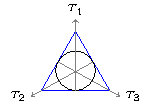
\includegraphics[width=0.48\columnwidth]{dalitz-tri}}
  % 
  \hfill
  % 
  \subbottom[Dalitzplottet med indtegnede resonansbånd. Det smalle røde viser $\alpha_{0}$, mens den bredde
  viser $\alpha_{1}$.]
  {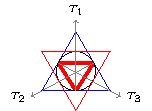
\includegraphics[width=0.48\columnwidth]{dalitz-band}}%
  \caption{}
  \label{fig:dalitz-triangle}
\end{figure}

\subsubsection{Symmetribetragtninger}
\label{sec:symbetragt}

Såfremt der ikke er nogen symmetribegrænsninger og henfaldsprodukterne ikke vekselvirker med
hinanden, vil matrixelementet være en konstant og henfaldet vil udelukkende afgøres af
faserummet. Dette svarer til statistisk henfald og vil give anledning til en flad fordeling
\cite{Fedorov}, hvilket vil være tilfældet ved direkte henfald.

Henfalder systemet i stedet via en resonans for derefter at henfalde til sluttilstanden, vil det ses
på plottet som et bånd. I forhold til den sekventielle henfaldsmodel og koincidensspektrene
forventes bånd svarende til energien af $\alpha_{0}$ og $\alpha_{1}$. Bredden af disse bånd vil være bestemt
af berylliumtilstandens bredde. $\alpha_{1}$-båndet bør derfor være væsentligt breddere, hvilket er
indtegnet på \cref{fig:dalitz-triangle}b. Dalitzplottet kan dermed bruges til at identificere
resonanser og bredden af disse.

$\alpha$-henfaldet er ikke et svagt henfald, så både spin og paritet skal være bevaret. Endvidere er
$\alpha$-partikler bosoner, så den samlede bølgefunktion skal være symmetrisk under ombytning af de tre
$\alpha$-partikler. På baggrund af disse bevarelseslove skal matrixelementet, og dermed Dalitzplottet,
være nul i visse områder. Denne udledning er foretaget i \cite{Fedorov} og resultatet ses på
\cref{fig:dalitz-0}.
%
\begin{figure}[h]
  \centering
  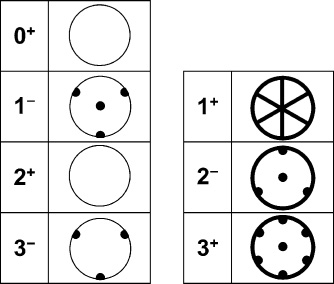
\includegraphics[width=0.3\columnwidth]{dalitz-zero}
  \caption{Områder af Dalitzplottet, hvor fordelingen skal være 0. }
  \label{fig:dalitz-0}
\end{figure}

Den generelle tendens viser, at for tilstandene med unaturlig paritet $\pi = (-1)^{J+1}$, dvs. i højre
kolonne, stiller symmetrien strenge krav til, hvor fordelingen skal være nul. Kravene til
tilstandene med naturlig paritet $\pi = (-1)^{J}$ er væsentligt mindre. Endvidere ses, at det
udelukkende er tilstande med unaturlig paritet, hvor fordelingen skal være nul langs hele randen.

Det er muligt at forklare effekten af $\alpha$-partiklernes bølgenatur på Dalitzplottet mere
intuitivt. Ud fra tre målte energier er der tre mulige måder, hvorpå man kan kombinere de tre
$\alpha$-partikler, således de danner \Be*. Dette svarer til, at der for hver konfiguration er tre
muligheder for hvilken partikel, der udsendes først.

Hvis \Be* tilstanden er smal, er kun en af konfigurationerne realisérbar. Dette svarer til
områderne, hvor $\alpha_{0}$-båndene skærer den indskrevne cirkel på \cref{fig:dalitz-triangle}b. Her er
kun én konfiguration mulig, da den mest energirige partikel nødvendigvis må være
$\alpha_{0}$-partiklen.

% Den første exciterede tilstand i beryllium er dog meget bred, så her vil der være mere end et bidrag
% som summeres. På \cref{fig:dalitz-triangle}b vil det svare til områderne hvor båndene krydser, da
% præcis i disse områder er flere konfigurationsmuligheder.

Den første exciterede tilstand i beryllium er meget bred. I områderne på
\cref{fig:dalitz-triangle}b, hvor $\alpha_{1}$-båndene krydser, vil der være mere end én sandsynlig
konfiguration.  Den endelige bølgefunktion er dermed en linearkombination af flere bølgefunktioner
og idet denne skal være symmetrisk, vil områderne, hvor båndene overlapper, svare til konstruktiv
interferens mellem de enkelte bølgefunktioner. 















\section{Data og databehandling}
\label{sec:dalitz-data}

Databehandlingen af dette er stort set tilsvarende den i \cref{sec:sek-data}. Eneste forskel er, at når
der blev fundet en koincidens, så blev Dalitzkoordinaterne udregnet. Hvis punktet lå uden for den
indskrevne cirkel, så blev det smidt væk.

\subsection{\SI{17.8}{\MeV}}
\label{sec:dalitz-178}


På \cref{fig:dalitz-1077} ses Dalitzplottet for trippel-$\alpha$ henfaldet fra den exciterede tilstand
ved \SI{17.8}{\MeV} i kulstof. %Som forventet er plotet symmetrisk. 

Båndene svarende til $\alpha_{0}$ ses ude ved kanten af cirklen, hvilket stemmer overens med, at de er
det meste energirige partikler i henfaldet. Som forventet er det smalle bånd svarende til at
berylliumresonansen er meget lang livet. Lidt under $\alpha_{0}$ ses også en struktur i dobbeltkoincidenserne,
der ligner lidt en klo. Dette skyldes tilfældige koincidenser, formentlig på grund af beamet. I
Dalitzplottet genfindes også den tidligere observerede tendens med stærk undertrykkelse af $\alpha_{0}$
når dobbeltkoincidenserne benyttes. 

\begin{figure}[t]
  \centering
  \subbottom[Dobbelkoincidenser]{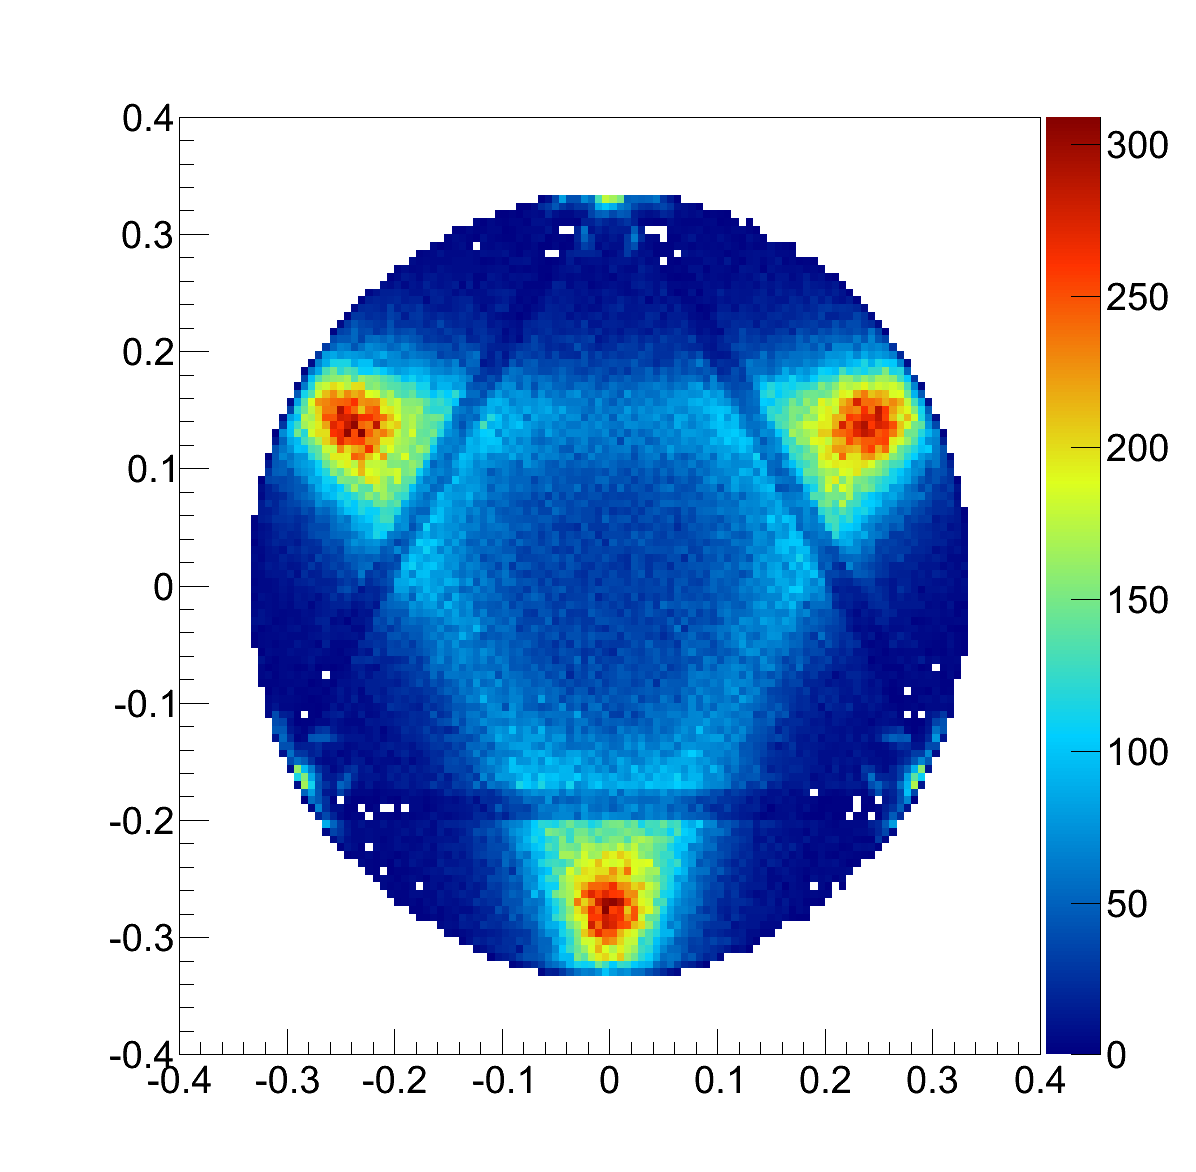
\includegraphics[width=0.46\columnwidth]{1077-Dalitz-D}}%
  \hfill
  \subbottom[Trippelkoincidenser]{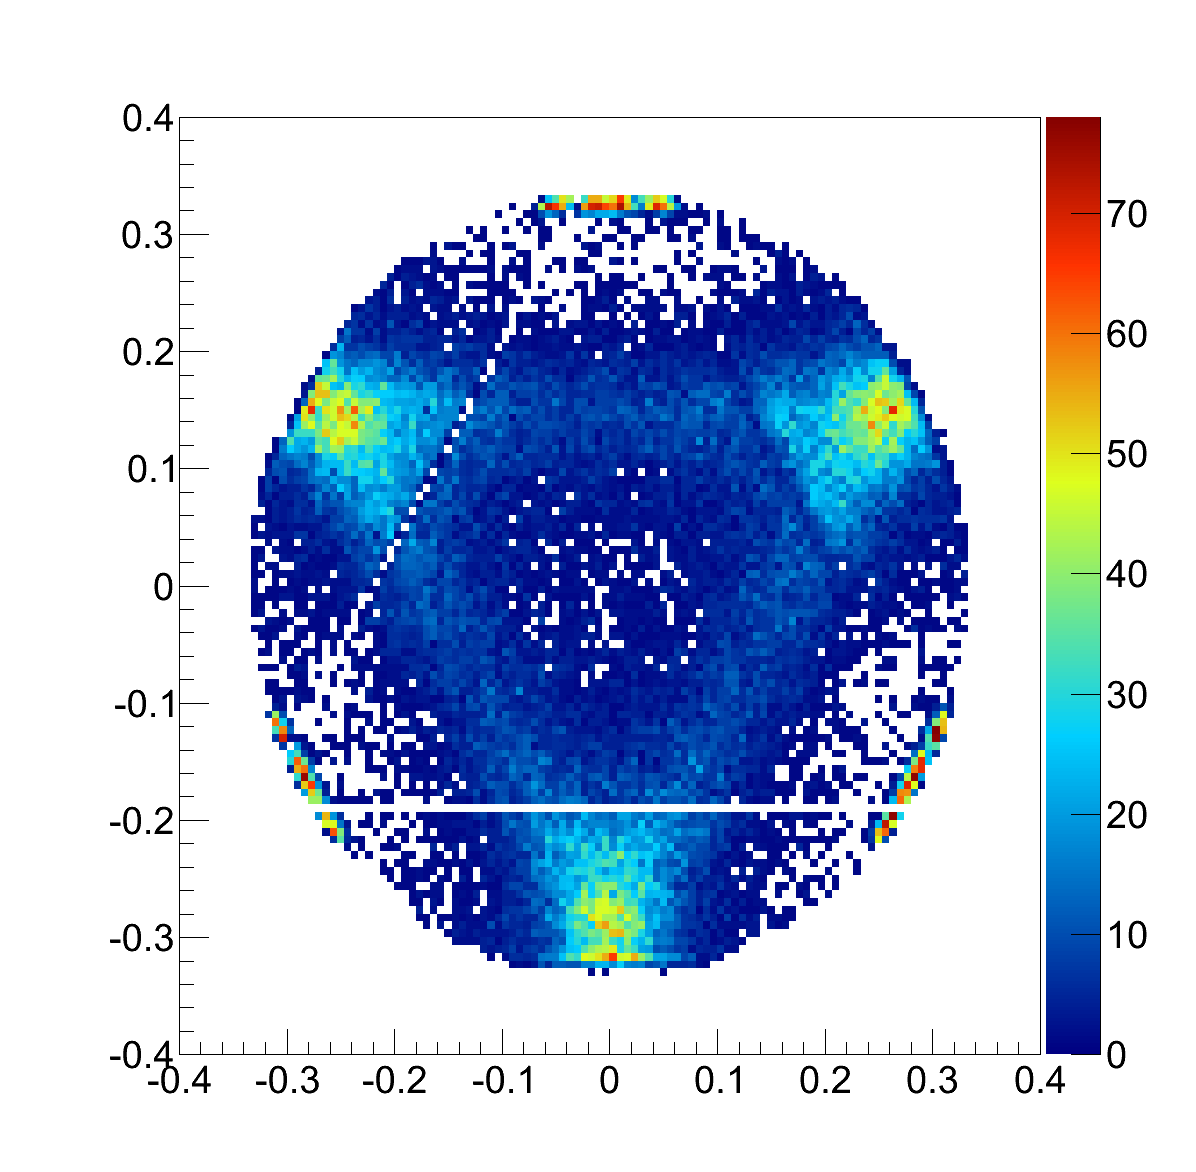
\includegraphics[width=0.46\columnwidth]{1077-Dalitz-T}}%
  \caption{Dalitzplot for $0^{+}$ tilstanden ved \SI{17.8}{\MeV} i kulstof.}
  \label{fig:dalitz-1077}
\end{figure}

Ved lidt lavere energi ses båndene for $\alpha_{1}$. Toppene ude ved sidderne og i bunden har den samme
struktur i de to plots, selv om toppene er mere fremtrædende når dobbeltkoincidenserne
benyttes. Dette skyldes, som tidligere diskuteret, at disse er bedre til at detektere $\alpha_{1}$. I
området mellem toppene er strukturen også den samme. Dobbelkoincidenserne har dog fordelen ved den
øgede datamængde, som får dens strukture til at adskille sig bedre fra baggrunden. Der er dog ingen
tvivl om at bredden af $\alpha_{1}$-båndet er væsentligt større end $\alpha_{0}$-båndet. 

Hvilken tilstand er så blevet populeret? Ud fra \cref{fig:dalitz-0} kan de to tilstande med naturlig
paritet $1^{-}$ og $3^{-}$ udelukkes, da disse kræver, at der er nulpunkter ved de steder
$\alpha_{1}$-båndet har maksima. Alle tilstandene med unaturlig paritet kræver at fordelingen er nul
langs hele randen, hvilket er hvor maksima for både $\alpha_{0}$- og $\alpha_{1}$-båndet befinder sig. Ud over
dette, stiller de også visse andre krav, som ikke heller ikke er opfyldt.

Dermed er antallet af kandidater reduceret til $0^{+}$ og $2^{+}$, for hvilke symmetrien stiller
samme krav. Der er desuden den mulighed, at det kan være en tilstand, som ikke er tabuleret i
\cite{Fedorov}. En videre analyse vil kræve simuleringer, hvilket er uden for tidsrammen af dette
projekt. Heldigvis er tilstanden tabuleret og ifølge \cite{States} er den
populerede tilstand en $0^{+}$ tilstand, hvilket stemmer smukt overens med resultaterne.
















